\section{The Short-Time Fourier Transform}
A signal in time contains information about the amplitude of the signal at specific times but does not hold any explicit informations about the frequencies. On the other hand, the Fourier transform of a signal contains information about a certain frequency but not at which time it appears.
\\ \\
From a musical point of view, let $f(t)$ be a piece of music describing the amplitude of the vibration of a speaker membrane in time, $t \in \mathbb{R}$. From this signal one is possibly able to detect the rythmical patterns of the music but probably not the melody or just single tones. On the other hand, the Fourier transform of $f$, $\mathcal{F}\{f(t)\}(\omega)$, will show the dominating frequencies of the piece of music from which one can detect the tones but not the duration of these. Therefore, neither the signal in time $f(t)$ nor the Fourier transform $F(\omega)$ in frequency contains all the relevant information in order to describe the signal.
\\
Figure \ref{fig:sine_STFT} is a follow-up from figure \ref{fig:sine_sum} and initially shows a sine wave of the form $f_1(t) = \sin(220\pi\cdot t) + \sin(440\pi\cdot t)$, which is the tone $A_2$ with frequency $110$ Hz and a single harmonic of $A_3$ with frequency $220$ Hz. After approximately 22 milliseconds the sine wave shifts to $f_2(t) = \sin(880\pi\cdot t) + \sin(1760\pi\cdot t)$, which is the tone $A_4$ with frequency $440$ Hz and a single harmonic of $A_5$ with frequency $880$ Hz. From a graph of a signal $f(t)$ similar to figure \ref{fig:sine_time_STFT} it is rather simple to determine the rythmical patterns of the music but one can not determine the frequencies. On the other hand, figure \ref{fig:sine_freq_STFT} shows the frequency spectrum of the sine waves, and it is quite obvious what the frequencies (and hence also tones) are, but no rythmical patterns can be determined from the frequency spectrum alone.

\begin{figure}[H]
	\centering
	\begin{subfigure}{0.49\textwidth}
		\centering
		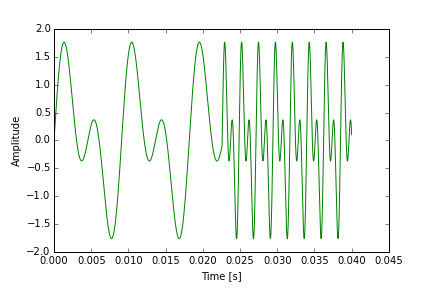
\includegraphics[width = \textwidth]{figures/sine_time_STFT.png}
		\caption{Two different tones represented in time.}
		\label{fig:sine_time_STFT}
	\end{subfigure}
	\begin{subfigure}{0.49\textwidth}
	\centering
		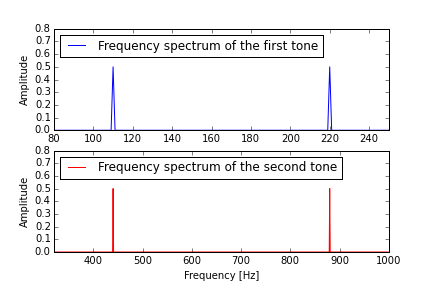
\includegraphics[width = \textwidth]{figures/sine_freq_STFT.png}
		\caption{Frequency spectrum of the tones.}
		\label{fig:sine_freq_STFT}
	\end{subfigure}
	\caption{Two tones represented in the time and frequency domain, respectively.}
	\label{fig:sine_STFT}
\end{figure}

Amazingly, the human ear and brain is able to perceive the bare signal $f$ and process it into a representation that provides simultaneous information about both time and frequency. This is actually known as music and is represented through the staff system shown in figure \ref{fig:cmajor} in chapter \ref{ch2}. The goal of time-frequency analysis (at least in this project) is to imitate the ear and create a joint time-frequency representation of a signal \cite{page 22, FTFA}. This is the incentive for the short-time Fourier transform (STFT), which may be thought of as the mathematical analog of the musical score \cite{page 37, FTFA}. The following is inspired by \cite{page 37, FTFA}.
\\ \\
The idea in the STFT is to obtain properties of a local frequency spectrum of $f$ by restricting it to an interval and taking the Fourier transform of this interval. $f$ is restricted on this interval by using a window function, which is close to 1 near the origin and decays towards zero at the edges, which is therefore a smooth cut-off function. The boundaries created by a sharp cut-off function will be interpreted by the Fourier transform as a discontinuity or an abrupt variation of the signal, which is obviously not desirable \cite{Davis}. The following definition of the STFT is inspired by the definition in \cite{page 37, FTFA} but has been adjusted to the definition of the Fourier transform used in this project. Also, $g$ is not assumed to take complex values as in \cite{page 37, FTFA}.

\begin{definition}[The Short-Time Fourier Transform]\label{def:stft}
Let $f,g \in \mathcal{L}^2(\mathbb{R}^d)$. For a fixed window function $g \neq 0$ the short-time Fourier transform of a function $f$ with respect to $g$ is defined as:
\begin{align}
V_gf(\tau,\omega) = \int_{\mathbb{R}^d} f(t) g(t - \tau) \text{e}^{-j \omega t} dt \quad \textnormal{for} \quad \tau,\omega \in \mathbb{R}^d.
\end{align}
\end{definition}

$V_gf(\tau,\omega)$ can be thought of as a measure for the amplitude of the frequency band near $\omega$ at time $\tau$. The window function $g$ is usually kept fixed, and $V_gf$ is considered to be a linear mapping from functions on $\mathbb{R}^d$ to functions on $\mathbb{R}^{2d}$, which is known as the \textit{time-frequency plane} for $d=1$ in signal analysis \cite{page 38, FTFA}. Definition \ref{def:stft} can be formulated for discrete-time systems.

\begin{definition}[The discrete Short-Time Fourier Transform]\label{def:stft_discrete}
Let $f,g\in\ell^2$. For a fixed window sequence $g\neq0$ the discrete short time Fourier transform of a sequence $f$ with respect to $g$ is defined as
\begin{align}
V_gf[n,\omega]=\sum_{m=-\infty}^{\infty}f[n+m]g[m]\mathrm{e}^{-j\omega t}.
\end{align}
\end{definition}
Figure \ref{fig:sliding_stft} illustrates how the STFT windows a signal.
\begin{figure}[H]
\centering
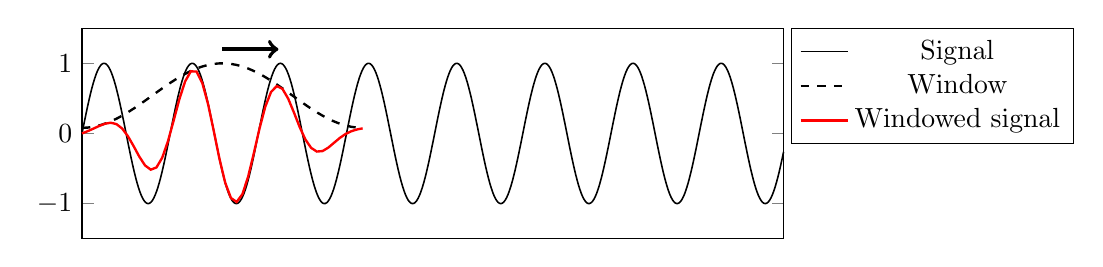
\begin{tikzpicture}
\begin{axis}[scale=1.3,
xtick=\empty,
xmin=0,
xmax=10,
ymin=-1.5,
ymax=1.5,
clip=false,
unit vector ratio*=1 1 1,
legend style={at={(axis cs:10.1,1.5)},anchor=north west}]
\addplot[samples=500,domain=0:10,line width=0.2mm]{sin(deg(5*x))};
\addplot[samples=50,domain=0:4,line width=0.3mm,dashed]{0.54-0.46*cos(deg(6.283/4*x))};
\addplot[samples=50,domain=0:4,line width=0.3mm,red]{(0.54-0.46*cos(deg(6.283/4*x)))*sin(deg(5*x))
};
\legend{Signal,Window,Windowed signal};
\draw[->,line width=0.5mm]{(axis cs:2,1.2)--(axis cs:2.8,1.2)};
\end{axis}
\end{tikzpicture}
\caption{Illustration of the discrete STFT windowing a signal. In this figure only a single window is shown, but the STFT windows and Fourier transforms the signal at several dicrete points in time.}
\label{fig:sliding_stft}
\end{figure}
Clearly, the STFT depends on how wide the window is:
\paragraph{A rather wide window} leads to good \textit{frequency resolutions}, and e.g. constant frequencies are thus clearly visible in the time-frequency plane. However, a spike will be blurred in the time-frequency plane as a wide window can't exactly determine at what time the spike occurs.
\paragraph{A rather narrow window} leads to good \textit{time resolutions}, which means that a spike is clearly visible at a given time, but constant frequencies are on the other hand blurred \cite{Davis}. \\ \\
This apparent tradeoff is due to the fact that it is fundamentally impossible to simultaneously have the complete information of a signal in both the time and frequency domain. This is a consequence of the Heisenberg uncertainty principle \cite{Wang}.

\subsection{The Heisenberg uncertainty principle}\label{sec:heisenberg}
The Heisenberg uncertainty principle comes from quantum physics, where it is impossible to simultaneously measure both the position and the momentum of a particle accurately since higher precision in one quantity implies lower precision in the other. This is also the case in the time and frequency domain, which the following lemma shows \cite{page 123, Wang}.

\begin{lemma}
\begin{align*}
\mathcal{F}\{x(at)\}(\omega) = \dfrac{1}{|a|}F\left(\dfrac{\omega}{a}\right)
\end{align*}
\end{lemma}

\begin{proof}
First, it is assumed that $a > 0$:
\begin{align*}
\mathcal{F}\{x(at)\}(\omega) = \int_{-\infty}^\infty x(at)e^{-j\omega t} dt = \int_{-\infty}^\infty x(u) e^{-j\omega \frac{u}{a}} d\left(\dfrac{u}{a}\right) = \dfrac{1}{a} \int_{-\infty}^\infty x(u) e^{-j\frac{\omega}{a} u} du = \dfrac{1}{a} F\left(\dfrac{\omega}{a}\right),
\end{align*}

where $u = at$, which means that $t = \frac{u}{a}$. Likewise, $\mathcal{F}\{x(-at)\}(\omega) = \dfrac{1}{a} X \left(- \dfrac{\omega}{a}\right)$, and therefore, if $a' = -a < 0$ then:
\begin{align*}
\mathcal{F}\{x(a't)\}(\omega) = \dfrac{1}{-a'} X\left(\dfrac{\omega}{a'}\right)
\end{align*}

with $u = a't$.
\end{proof}

Therefore, this lemma shows that if a time function $x(t)$ is expanded, then its spectrum $F(\omega)$ is compressed, and if $x(t)$ is compressed, then $F(\omega)$ is conversely expanded. A rather extreme example is an impulse, which is concentrated within a short time range, and its Fourier transform is a constant, $\mathcal{F}\{\delta(t)\}(\omega) = 1$. Conversely, a constant, which is spread in time, has an impulse as its Fourier transform, $\mathcal{F}\{1\}(\omega) = \delta(t)$. This is the background for the Heisenberg uncertainty principle, which is stated with some concepts from probability theory. The function $p_x(t)$
\begin{align*}
p_x(t) = \dfrac{|x(t)|^2}{\|x(t)\|^2} = \dfrac{|x(t)|^2}{\int_{-\infty}^\infty |x(t)|^2 dt}
\end{align*}

is a probability density function since it satisfies the conditions
\begin{align*}
p_x(t) > 0 \quad \text{and} \quad \int_{-\infty}^\infty p_x(t) dt = 1.
\end{align*}

The variance of $p_x(t)$, $\sigma_t^2$, is a measure of the dispersion of $x(t)$:
\begin{align*}
\sigma_t^2 = \int_{-\infty}^\infty (t - \mu_t)^2 p_x(t) dt = \dfrac{1}{\|x(t)\|^2} \int_{-\infty}^\infty (t - \mu_t)^2 |x(t)|^2 dt,
\end{align*}

where $\mu_t$ is the mean of $p_x(t)$:
\begin{align*}
\mu_t = \int_{-\infty}^\infty t p_x(t) dt = \dfrac{1}{\|x(t)\|^2} \int_{-\infty}^\infty t |x(t)|^2 dt.
\end{align*}

Similarly, the dispersion of the spectrum of the signal can be measured as:
\begin{align*}
\sigma_\omega^2 &= \dfrac{1}{\|X(\omega)\|^2} \int_{-\infty}^\infty (\omega - \mu_\omega)^2 |X(\omega)|^2 d\omega, \\
\mu_\omega &= \dfrac{1}{\|X(\omega)\|^2} \int_{-\infty}^\infty \omega |X(\omega)|^2 d\omega.
\end{align*}

Note that
\begin{align*}
\|x(t)\|^2 = \int_{-\infty}^\infty |x(t)|^2 dt = \dfrac{1}{2\pi} \int_{-\infty}^\infty |X(\omega)|^2 d\omega = \dfrac{1}{2\pi} \|X(\omega)\|^2
\end{align*}

due to theorem \ref{theo:Plancherel} \martin{Ikke helt sikker på, at dette gælder, og det er vigtigt i forhold til beviset (se også næste kommentar). \textregistered}. Now the uncertainty principle can be stated as the following theorem.

\begin{theorem}
Let $\mathcal{F}\{x(t)\}(\omega) = X(\omega)$ be the spectrum of a given function $x(t)$ with variances $\sigma_\omega^2$ and $\sigma_t^2$, respectively. Then:
\begin{align*}
\sigma_t^2 \sigma_\omega^2 \geq \dfrac{1}{16 \pi^2}.
\end{align*}
\end{theorem}

\begin{proof}
It is assumed that $\mu_t = \mu_\omega = 0$ without loss of generality, and then
\begin{align} \label{eq:Heis_proof}
\sigma_t^2 \sigma_\omega^2 &= \dfrac{1}{\|x(t)\|^2 \|X(\omega)\|^2} \int_{-\infty}^\infty |tx(t)|^2 dt \int_{-\infty}^\infty |\omega X(\omega)|^2 d\omega \\
&= \dfrac{2\pi}{\|x(t)\|^4} \int_{-\infty}^\infty |tx(t)|^2 dt \int_{-\infty}^\infty |\omega X(\omega)|^2 d\omega.
\end{align}

Due to property (c) in theorem \ref{theorem:fund_sym_Fourier} and Parseval's equation it is seen that
\begin{align*}
\dfrac{1}{j} \mathcal{F}\{x'(t)\}(\omega) = \omega X(\omega)
\end{align*}

and \martin{Dette holder ikke helt på grund af vores definition af Fourier-transformationen, og jeg kan ikke helt gennemskue, hvordan ligningen skal skrives rigtigt. \textregistered}
\begin{align*}
\int_{-\infty}^\infty |\omega X(\omega)|^2 d\omega = \dfrac{1}{4\pi^2} \int_{-\infty}^\infty |x'(t)|^2 dt.
\end{align*}

Therefore, \eqref{eq:Heis_proof} becomes:
\begin{align} \label{eq:Heis_proof2}
\sigma_t^2 \sigma_\omega^2 &= \dfrac{1}{4\pi^2 \|x(t)\|^4} \int_{-\infty}^\infty |tx(t)|^2 dt \int_{-\infty}^\infty | x'(t)|^2 dt \nonumber \\
&\geq \dfrac{1}{4\pi^2 \|x(t)\|^4} \left[ \int_{-\infty}^\infty t \overline{x}(t)x'(t) dt \right]^2,
\end{align}

where the last inequality follows from the Cauchy-Schwarz inequality and $\overline{x}(t)$ is the complex conjugate of $x(t)$. Since
\begin{align*}
\left[ |x(t)|^2 \right]' = \left[ x(t) \overline{x}(t) \right]' = x'(t) \overline{x}(t) + \overline{x}'(t) x(t) = 2 \operatorname{Re} \left[ x'(t) \overline{x}(t) \right] \leq 2 x'(t) \overline{x}(t)
\end{align*}

then $\overline{x}(t) x'(t)$ in the integrand in \eqref{eq:Heis_proof2} can be replaced by $\left[ |x(t)|^2 \right]'/2$:
\begin{align} \label{eq:Heis_proof3}
\sigma_t^2 \sigma_\omega^2 \geq \dfrac{1}{4\pi^2 \|x(t)\|^4} \left[ \int_{-\infty}^\infty \dfrac{t \left[ |x(t)|^2 \right]'}{2} dt \right]^2 = \dfrac{1}{4 \cdot 4\pi^2 \|x(t)\|^4} \left[ \int_{-\infty}^\infty t \left[ |x(t)|^2 \right]' dt \right]^2.
\end{align}

The integral is integrated by parts:
\begin{align*}
\int_{-\infty}^\infty t \left[ |x(t)|^2 \right]' dt = \left[ t |x(t)|^2 \right]_{t=-\infty}^\infty - \int_{-\infty}^\infty |x(t)|^2 dt = - \int_{-\infty}^\infty |x(t)|^2 dt
\end{align*}

where it has been assumed that $\lim_{|t| \to \infty} t |x(t)|^2 = 0$. This result is substituted into \eqref{eq:Heis_proof3}, which then yields:
\begin{align*}
\sigma_t^2 \sigma_\omega^2 &\geq \dfrac{1}{4 \cdot 4\pi^2 \|x(t)\|^4} \left[ \int_{-\infty}^\infty t \left[ |x(t)|^2 \right]' dt \right]^2 \\
&= \dfrac{1}{4 \cdot 4\pi^2 \|x(t)\|^4} \left[ - \int_{-\infty}^\infty |x(t)|^2 dt \right]^2 \\
&= \dfrac{1}{4 \cdot 4\pi^2 \|x(t)\|^4} \left[ \int_{-\infty}^\infty |x(t)|^2 dt \right]^2 \\
&= \dfrac{\|x(t)\|^4}{16\pi^2 \|x(t)\|^4} = \dfrac{1}{16\pi^2}.
\end{align*}
\end{proof}

Therefore, the optimal variance in time and frequency satifies the relation $\sigma_t^2\sigma_\omega^2 = \frac{1}{16\pi^2}$ \martin{Mangler i dette afsnit: beviset skal tilpasses vores definition af Fourier-transformationen. Derudover mangler vi minimum én figur, der illustrerer STFT'en. \textregistered}.